\documentclass[a4paper,12pt]{article} 

%%% Работа с русским языком
\usepackage{cmap}					% поиск в PDF
\usepackage{mathtext} 				% русские буквы в фомулах
\usepackage[T2A]{fontenc}			% кодировка
\usepackage[utf8]{inputenc}			% кодировка исходного текста
\usepackage[english,russian]{babel}	% локализация и переносы

%%% Дополнительная работа с математикой
\usepackage{amsmath,amsfonts,amssymb,amsthm,mathtools, gensymb} % AMS
\usepackage{icomma} % "Умная" запятая: $0,2$ --- число, $0, 2$ --- перечисление

%%Таблица
\usepackage[table,xcdraw]{xcolor}
\usepackage{caption}
\usepackage{subcaption}
\usepackage{floatrow}
\floatsetup[table]{capposition=top}
\floatsetup[wrapfigure]{capposition=bottom}


%% Номера формул
\mathtoolsset{showonlyrefs=true} % Показывать номера только у тех формул, на которые есть \eqref{} в тексте.

%% Шрифты
\usepackage{euscript}	 % Шрифт Евклид
\usepackage{mathrsfs} % Красивый матшрифт

%% Свои команды
\DeclareMathOperator{\sgn}{\mathop{sgn}}

%% Перенос знаков в формулах (по Львовскому)
\newcommand*{\hm}[1]{#1\nobreak\discretionary{}
{\hbox{$\mathsurround=0pt #1$}}{}}

%% Стиль страницы
\usepackage{fancyhdr}

%% Для рисунков
\usepackage{graphicx}
\usepackage[export]{adjustbox}
\usepackage{float}
\usepackage{ragged2e}
\usepackage{wrapfig}

%Отступы и поля 
\textwidth=20cm
\oddsidemargin=-2cm
\topmargin=-2cm
\textheight=25cm

\pagestyle{fancy}
\begin{document}
\begin{titlepage}
\begin{center}
%\vspace*{1cm}
\large{\small ФЕДЕРАЛЬНОЕ ГОСУДАРСТВЕННОЕ АВТОНОМНОЕ ОБРАЗОВАТЕЛЬНОЕ\\ УЧРЕЖДЕНИЕ ВЫСШЕГО ОБРАЗОВАНИЯ \\ МОСКОВСКИЙ ФИЗИКО-ТЕХНИЧЕСКИЙ ИНСТИТУТ\\ (НАЦИОНАЛЬНЫЙ ИССЛЕДОВАТЕЛЬСКИЙ УНИВЕРСИТЕТ)\\ ФАКУЛЬТЕТ АЭРОКОСМИЧЕСКИХ ТЕХНОЛОГИЙ}
\vfill
\line(1,0){430}\\[1mm]
\huge{Лабораторная 7}\\
\huge\textbf{Изнаночка наших любимых плюсов}\\
\line(1,0){430}\\[1mm]
\vfill
\begin{flushright}
\normalsize{Рогозин Владимир}\\
\normalsize{\textbf{Группа Б03-106}}\\
\end{flushright}
\end{center}
\end{titlepage}
\fancyhead[L] {Лабораторная 7}

\textbf{Пункт 1: Методы и поля классов в листинге}

Первым пунктом посмотрим на классы, их поля и методы. Напишем класс с парой полей, конструкторов, методов, посмотрим как формируются их названия. 
\begin{figure}[H]\label{fig: Код генерация названий}
    \centering
    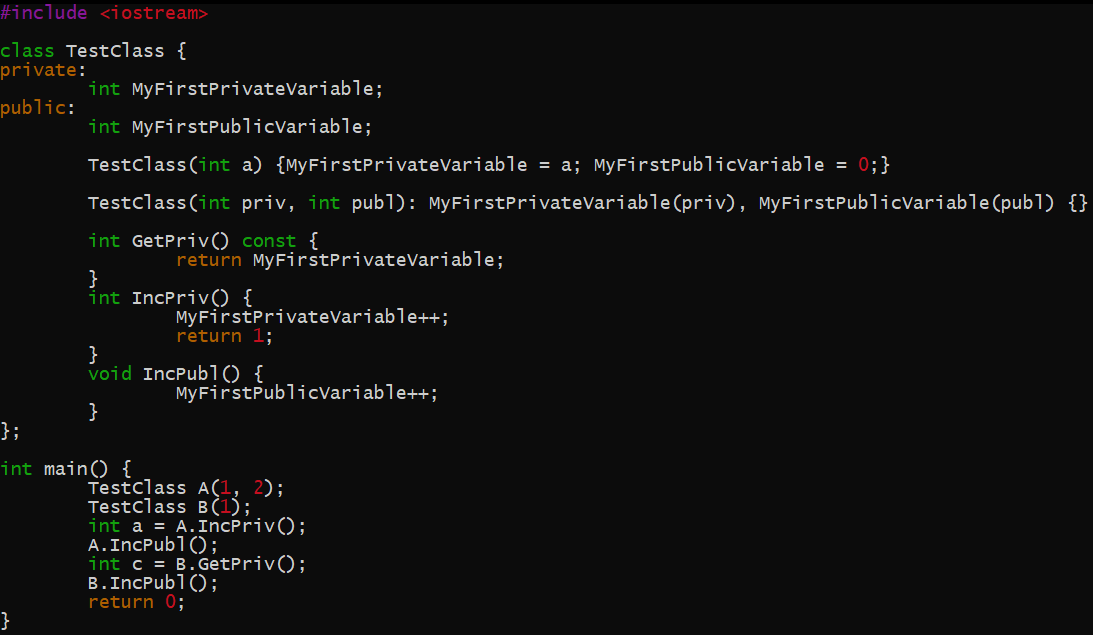
\includegraphics[width = \textwidth]{Код генерация названий.png}
    \caption{Простейший класс с двумя конструкторами, методами и полями}
\end{figure}
Сгенерируем листинг, посмотрим на названия методов в листинге.

\begin{figure}[H]\label{fig: Названия конструкторов}
    \subfloat[Первый конструктор]{
    \begin{minipage}[t]{0.4\textwidth}
        \centering
        
\includegraphics[scale = 0.6]{Название конструктор1.png}
    \end{minipage}}
    \subfloat[Второй конструктор]{
    \begin{minipage}[t]{0.4\textwidth}
        \centering
        
\includegraphics[scale = 0.6]{Название конструктор2.png}
    \end{minipage}}
\end{figure}
\begin{figure}[H]\label{fig: Вызов конструкторов листинг}
    \centering
    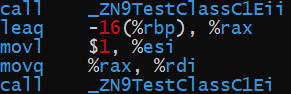
\includegraphics{Вызов конструкторов листинг.png}
    \caption{Вызов конструктора}
\end{figure}

В названиях конструкторов сначала идёт непонятная приписка \_ZN9, затем идёт название класса (по сути название функции, так как это конструктор), потом C2E, затем приписка i и ii соответственно (int и int int), что явно показывает типы аргументов функции.

Примечательно то, что при вызове конструктора его название передаётся не таким, как оно записано при объявлении функции (тaм С2 в названии, а не C1). Как будто компилятор сам переименовал функцию, иначе бы он не смог создать экземпляр класса. Далее смотрим на методы класса.

\begin{figure}[H]\label{fig: Конст и неконст методы}
    \subfloat[Константный метод]{
    \begin{minipage}[t]{0.4\textwidth}
        \centering
        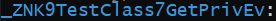
\includegraphics[scale = 0.6]{Название конст метод.png}
    \end{minipage}}
    \subfloat[Неконстантный метод]{
    \begin{minipage}[t]{0.4\textwidth}
        \centering
        
\includegraphics[scale = 0.6]{Название неконст метод.png}
    \end{minipage}}
\end{figure}
Теперь два метода, оба не принимают аргументов, один из которых const. Начало имени такое же, только в константном методе добавляется буква K (будто бы хотели написать Konst ха-ха). После этого идёт название класса, цифра 7 и название метода. После названия функции, как и в случае с конструкторами, идёт буква E, потом v, что означает отсутствие аргументов функции. 
\begin{figure}[H]\label{fig: Неконст метод}
    \centering
    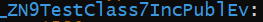
\includegraphics{Название неконст метод1.png}
    \caption{Неконстантный метод}
\end{figure}
В последнем методе все как и в предыдущих. Стоит ещё отметить, что в названиях функций никаким образом не указано что они должны (или ничего не должны) возвращать, указаны только типы данных аргументов функции.  

\textbf{Пункт 2: Как же он узнаёт с каким экземпляром класса работать?}

В этом пункте, так как метод класса это просто функция, посмотрим как она понимает какой экземпляр класса её вызывает. Для этого возьмём программу с прошлого пункта, посмотрим на примере конструктора. Ниже приведён его листинг.
\begin{figure}[H]\label{fig: Листинг конструктора и его вызова}
    \subfloat[Листинг вызова конструктора]{
    \begin{minipage}[t]{0.4\textwidth}
        \centering
        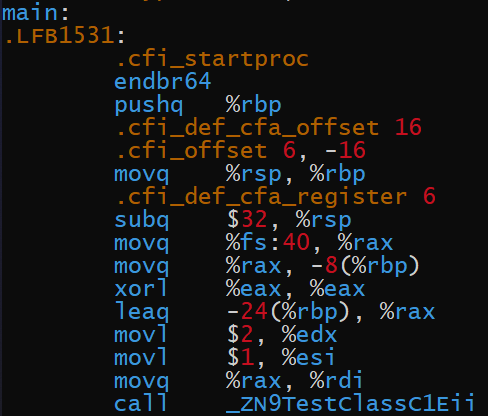
\includegraphics[scale = 0.51]{Вызов конструктора листинг.png}
    \end{minipage}}
    \subfloat[Листинг конструктора]{
    \begin{minipage}[t]{0.4\textwidth}
        \centering
        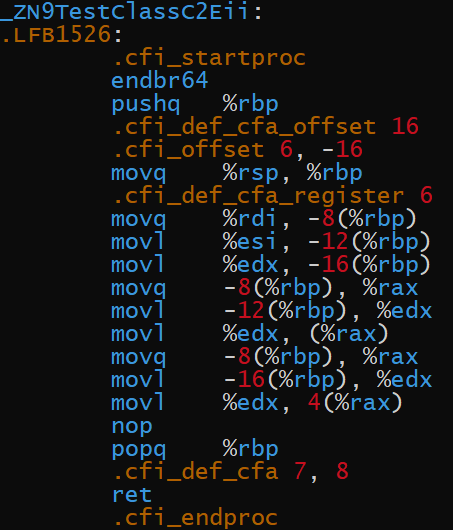
\includegraphics[scale = 0.4]{Неявная передача экземпляра класса.png}
    \end{minipage}}
\end{figure}
Видим, что при вызове метода класса неявным аргументом в функцию передаётся адрес того экземпляра класса, который вызвал этот метод. Передаётся адрес ячейки памяти через регистр $rdi$, именно таким образом машина понимает о каком именно объекте идёт речь.

\newpage
\textbf{Пункт 3: Раскрываем тайну загадочного слова \textit{this}}

Создадим функцию, использующую \textit{this}.
\begin{figure}[H]\label{fig: This код}
    \centering
    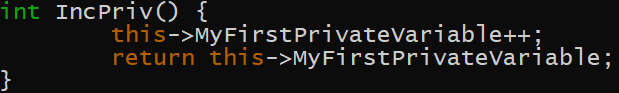
\includegraphics[width = 0.8\textwidth]{This функция код.png}
    \caption{Функция с \textit{this}}
\end{figure}
Теперь смотрим на её листинг.
\begin{figure}[H]\label{fig: This листинг}
    \centering
    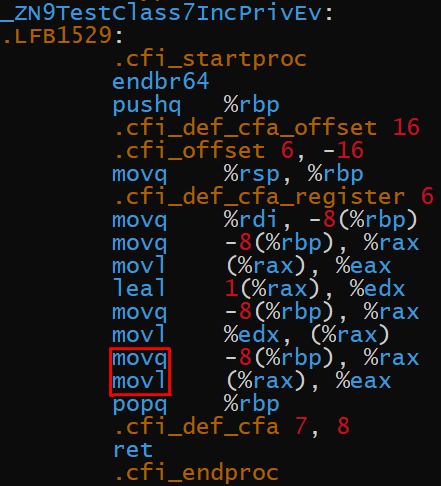
\includegraphics[width = 0.5\textwidth]{This функция листинг.png}
    \caption{Листинг функции выше}
\end{figure}
Из ассемблерного листинга видно, что \textit{this} работает как указатель, который в данном случае, чтобы функция вернула значение поля экземпляра класса, передаёт адрес объекта, потом по этому адресу уже берётся значение переменной конкретного экземпляра класса, и функция возвращает это значение.  

\textbf{Пункт 4: Конструкторы и деструкторы}

Посмотрим где и как вызываются конструкторы/деструкторы для локальных, глобальных, а также переменных, созданных в куче.

Сначала разберёмся с локальными переменными. При вызове конструктор принимает ещё один неявный аргумент -- адрес ячейки памяти где будет храниться объект (а точнее его первое поле). Передаётся этот адрес через регистр \textit{rdi}. С деструктором также, он дополнительно принимает адрес экземпляра класса, и если было какое-либо выделение памяти, то освобождает её.  

Если создавать объект в куче, то ситуация такая же, только на вход конструктору/деструктору приходит адрес памяти, которая выделяется в куче.

Деструкторы вызываются в порядке, обратном конструкторам. Если экземпляр находится в куче, то сначала вызывается деструктор, затем срабатывает \textit{delete} (если он конечно присутствует в коде).
\begin{figure}[H]\label{fig: Конструктор деструктор код}
    \centering
    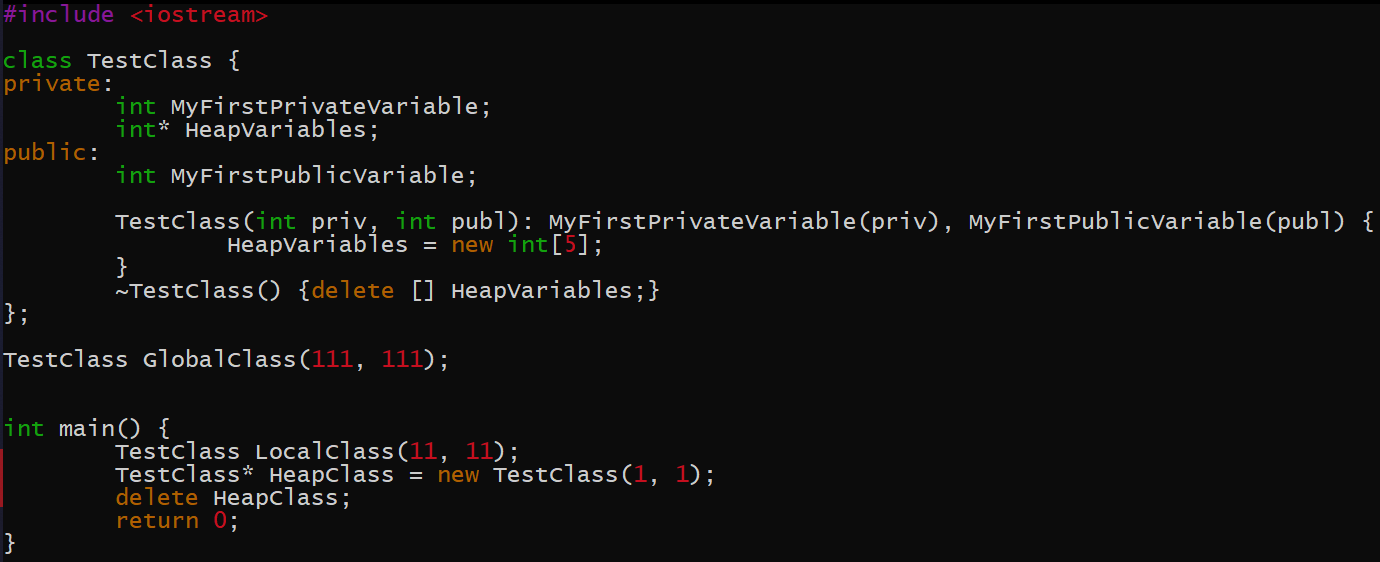
\includegraphics[width = 0.9\textwidth]{Конструктор деструктор код.png}
    \caption{Код программы}
\end{figure}
\begin{figure}[H]\label{fig: Листинг конструктора и деструктора}
    \subfloat[Листинг конструктора]{
    \begin{minipage}[t]{0.45\textwidth}
        \centering
        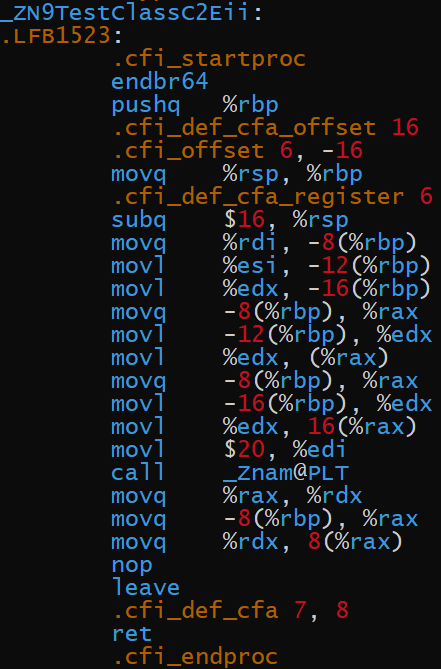
\includegraphics[scale = 0.55]{Конструктор.png}
    \end{minipage}}
    \subfloat[Листинг деструктора]{
    \begin{minipage}[t]{0.55\textwidth}
        \centering
        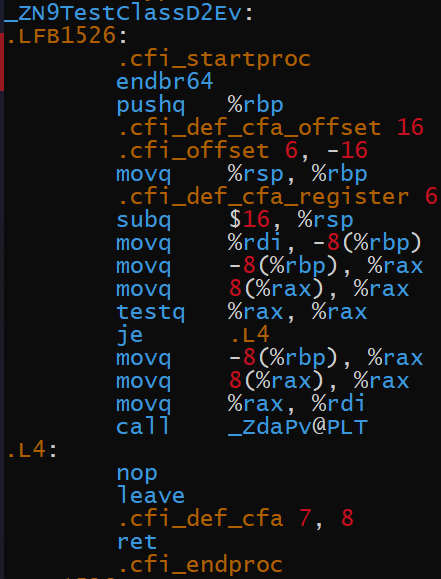
\includegraphics[scale = 0.63]{Деструктор.png}
    \end{minipage}}
\end{figure}
\newpage  

С глобальной переменной всё чуть иначе. Она, как и положено, объявляется в начале листинга. Но сам вызов конструктора и деструктора описан в конце листинга, после \textit{main'}а, так ещё и вызываются дополнительные непонятные функции. Конструктор вызывается как функция с помощью команды \textit{call}, а деструктор, как обычная переменная, кладётся в регистр $rdi$ и, судя по всему, потом с этим регистром что-то делает непонятная функция, которая вызывается после. 
\begin{figure}[H]\label{fig: Глобальный класс листинг}
    \subfloat[Объявление глобальной переменной]{
    \begin{minipage}[t]{0.5\textwidth}
        \centering
        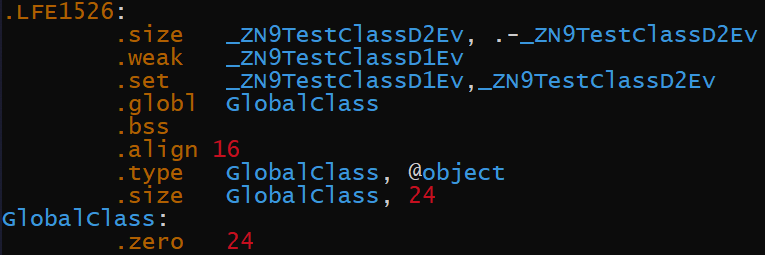
\includegraphics[scale = 0.4]{Объявление глобального класса.png}
    \end{minipage}}
    \subfloat[Вызов конструктора и деструктора]{
    \begin{minipage}[t]{0.55\textwidth}
        \centering
        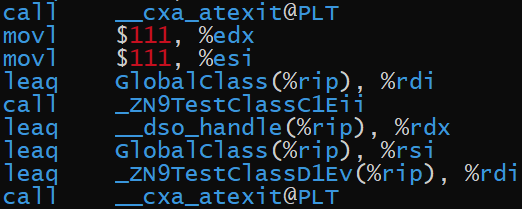
\includegraphics[scale = 0.486]{Конструктор деструктор глобального класса.png}
    \end{minipage}}
\end{figure}
Ещё стоит отметить, что если поля идут в порядке \textit{int}, \textit{int*}, \textit{int}, то, так как размер указателя равен 8-ми байтам, идёт выравнивание байтов, и каждому \textit{int'}у выделяется не 4, а 8 байт, всего один объект занимает 24 байта. если же поля идут в порядке \textit{int*}, \textit{int}, \textit{int}, то тогда каждой целочисленной переменной выделяется 4 байта и суммарное место, занимаемое экземпляром класса, сокращается до 16 байтов. То есть, записывая поля класса в правильном порядке, можно сэкономить немалое количество памяти.

\textbf{Пункт 5: Инкапсуляция. \textit{Public} и \textit{private} поля и методы}

Посмотрим как выглядит инкапсуляция в листинге. Для этого добавим приватный метод, сгенерируем листинг.
\begin{figure}[H]\label{fig: Приватные поля и методы код}
    \centering
    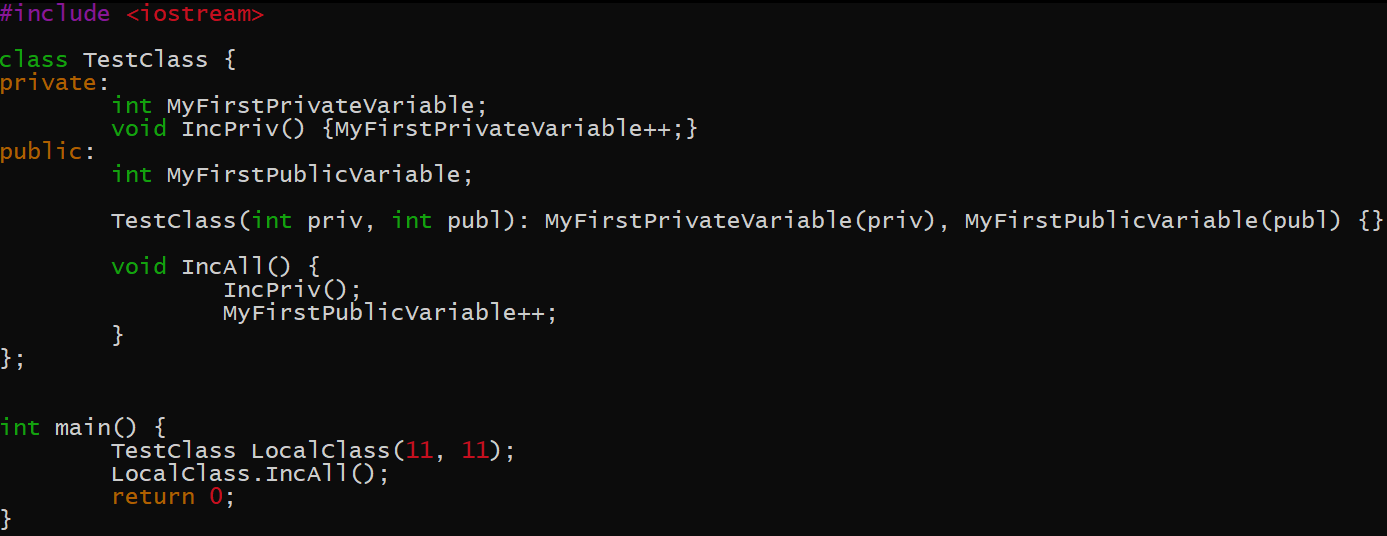
\includegraphics[width = 0.9\textwidth]{Приватные публичные поля код.png}
    \caption{Класс с приватным полем и методом}
\end{figure}
Из листинга приватного метода который меняет \textit{private} поле  видно, что с точки зрения ассемблера разницы никакой между \textit{private} и \textit{public} нету. Метод меняет поле точно также, как если бы оно было публичным. В функцию неявно передаётся указатель на объект, затем она получает доступ к любому, будь то \textit{private} или \textit{public}, полю.    
\begin{figure}[H]\label{fig: Приватные поля и методы листинг}
    \centering
    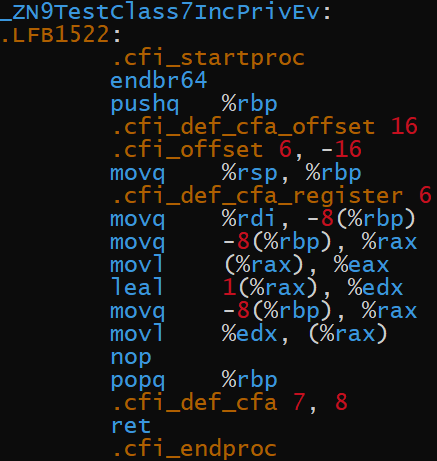
\includegraphics[width = 0.5\textwidth]{Приватные публичные поля листинг.png}
    \caption{Листинг \textit{private} функции, меняющей \textit{private} поле}
\end{figure}

\textbf{Пункт 6: Наследование}

Напишем некоторую иерархию классов, затем создадим экземпляр дочернего класса и посмотрим, как раскрываются конструкторы и в каком порядке лежат в памяти поля. 
\begin{figure}[H]\label{fig: Наследование код}
    \centering
    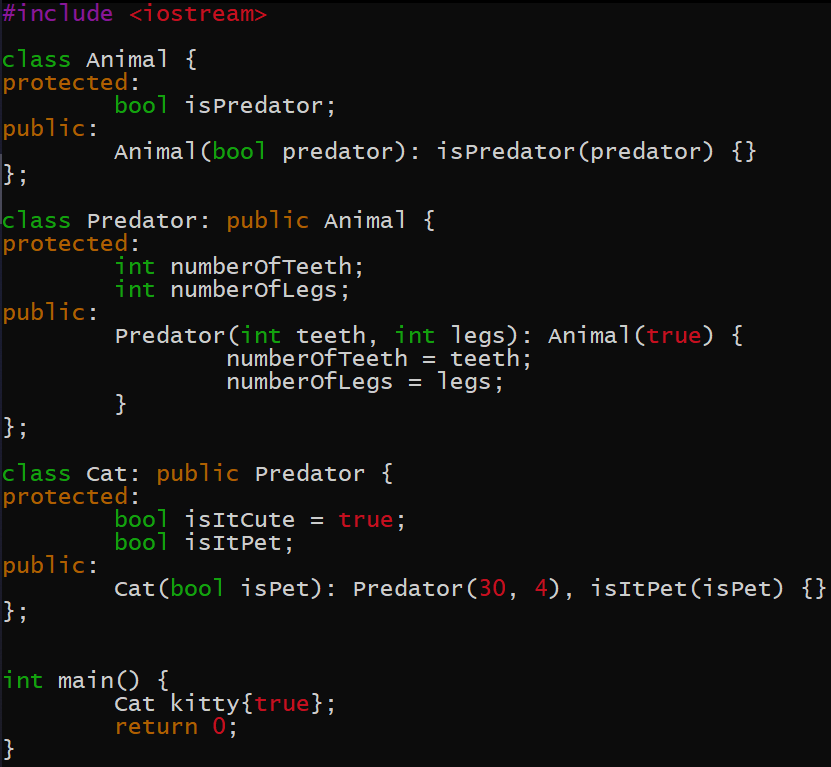
\includegraphics[width = 0.5\textwidth]{Наследование код.png}
    \caption{Код программы}
\end{figure}
\begin{figure}[H]\label{fig: конструкторы Predator и Cat}
    \subfloat[Конструктор класса Predator]{
    \begin{minipage}[t]{0.5\textwidth}
        \centering
        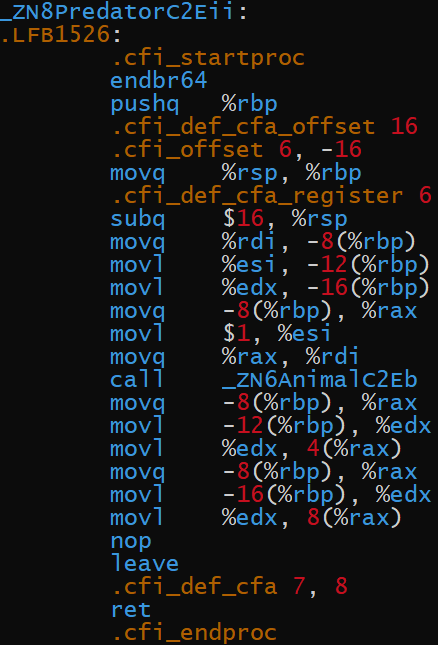
\includegraphics[scale = 0.5]{Конструктор Predator.png}
    \end{minipage}}
    \subfloat[Конструктор класса Cat]{
    \begin{minipage}[t]{0.5\textwidth}
        \centering
        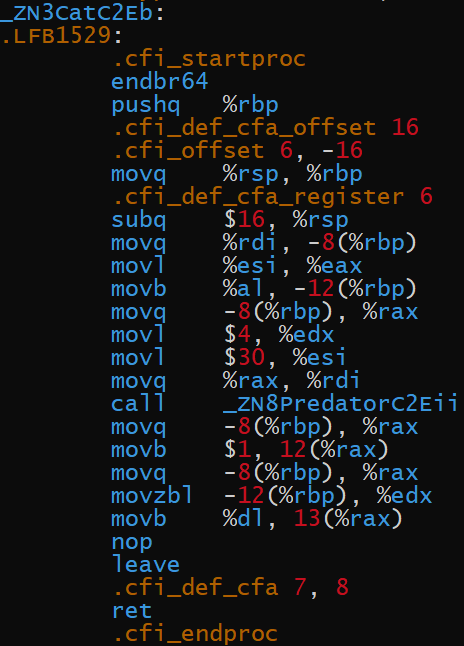
\includegraphics[scale = 0.5]{Конструктор Cat.png}
    \end{minipage}}
\end{figure}
Из листинга видим, что в конструкторе дочернего класса сначала вызывается конструктор родительского, а только после этого инициализируются поля дочернего класса. И поэтому в памяти сначала будут лежать поля базового класса, затем дочернего ему класса, затем дочернего дочернего и так далее до класса, экземпляр которого создаётся.
Это также объясняет порядок срабатывания конструкторов -- от базового и вниз по иерархии.

\textbf{Пункт 7: Откуда же полиморфизм}

Ну на этот вопрос теперь ответить не сложно. Возвращаясь к первому пункту этой лабы, понимаем, что названия функций, которые генерирует компилятор, включают в себя информацию о типах данных которые принимают функции в качестве аргументов. Таким образом, функция то не только название, но и аргументы, которые она принимает. Отсюда и получаем полиморфизм.

\textbf{Пункт 8: \textit{Static} поля и методы}

Посмотрим как выглядят \textit{static} поля и методы в ассемблере. Для этого добавим в класс такое поле и метод. Код приведён ниже. Сгенерируем листинг и проанализируем его.

Из листинга видим, что статиковые поля это что-то среднее между глобальными переменными и нестатиковыми полями класса. Объявляется такая переменная как глобальная, но в названии указана принадлежность к конкретному классу, поэтому можно создавать в разных классах статические переменные с одинаковым названием. Компилятор сам отслеживает законность/незаконность доступа к переменной вне класса (публичное ли поле или нет). Хранится, понятное дело, одна копия поля для всех экземпляров класса, статический метод, который есть обычная функция, обращается к этому полю как к глобальной переменной, поэтому при вызове этого метода нет нужды передавать адрес объекта, который вызывал статический метод -- адрес и не передаётся, а значит \textit{static} метод не может взаимодействовать с нестатическими полями и методами класса.

\begin{figure}[H]\label{fig: Статические поля и методы код}
    \centering
    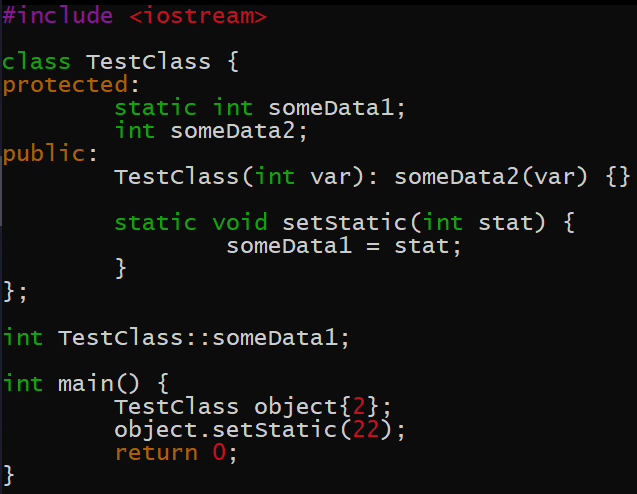
\includegraphics[width = 0.6\textwidth]{Статик переменные код.png}
    \caption{Класс со статическим полем и методом}
\end{figure}

\begin{figure}[H]\label{fig: Статическое поля листинг}
    \centering
    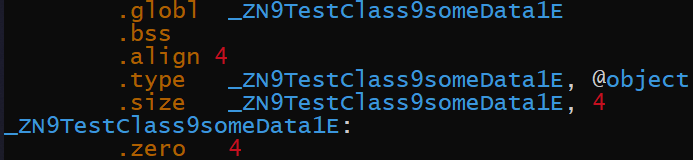
\includegraphics[width = 0.6\textwidth]{Статическое поле листинг.png}
    \caption{Статическое поле листинг}
\end{figure}

\begin{figure}[H]\label{fig: Статический методы листинг}
    \centering
    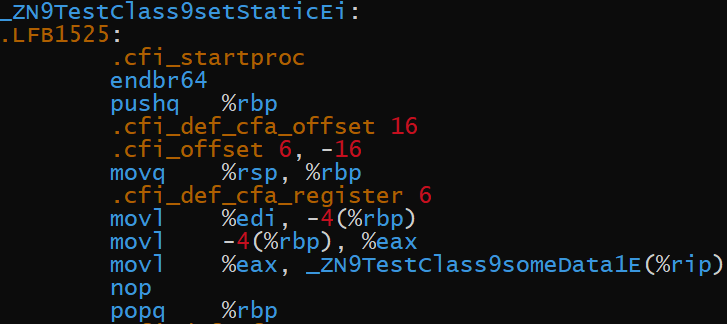
\includegraphics[width = 0.6\textwidth]{Статический метод листинг.png}
    \caption{Статический метод листинг}
\end{figure}
\newpage

\textbf{Пункт 9: Перегруженные операторы}

Перегрузим оператор сложения и посмотрим как он выглядит в ассемблерном листинге.
\begin{figure}[H]\label{fig: Оператор сложения код}
    \centering
    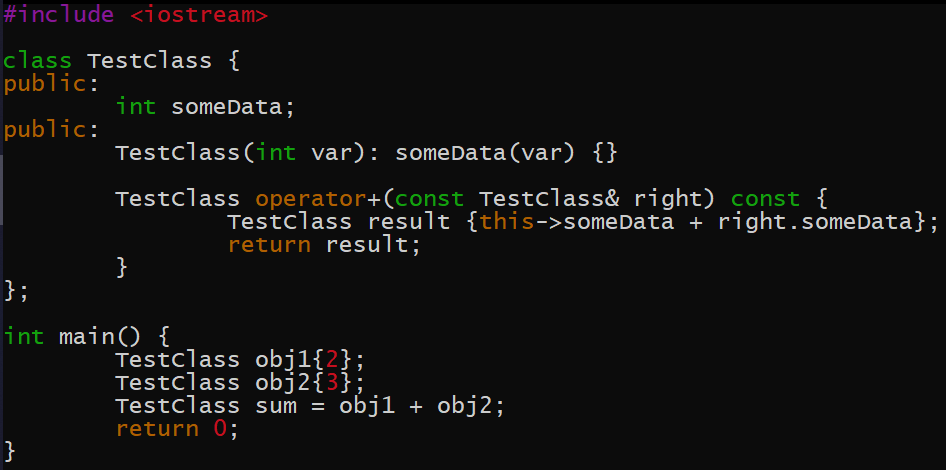
\includegraphics[width = 0.65\textwidth]{Оператор сложения код.png}
    \caption{Перегрузка оператора}
\end{figure}
\begin{figure}[H]\label{fig: Оператор сложения листинг}
    \centering
    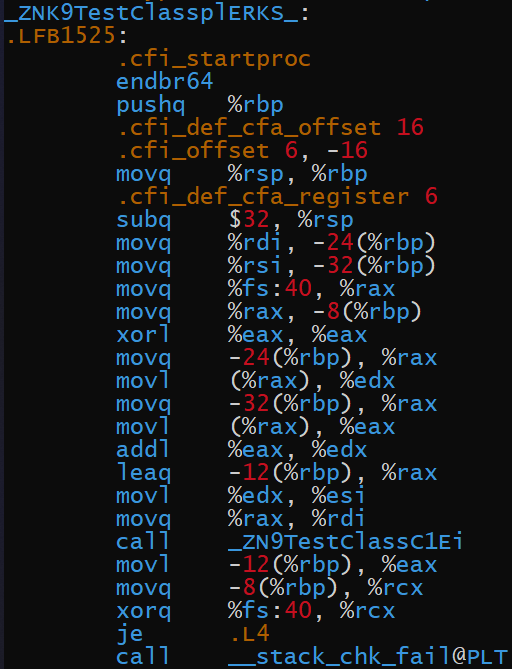
\includegraphics[width = 0.45\textwidth]{Оператор сложения листинг.png}
    \caption{Листинг перегруженного оператора}
\end{figure}
Вызываются операторы как функции, и из листинга видно, что это действительно просто функции. В названии функции также указано имя оператора (\textit{pl} означает плюс), а также типы данных аргументов.
\newpage

\textbf{Пункт 10: Шаблоны}

В этом пункте посмотрим на шаблонизацию функций и классов.
\begin{figure}[H]\label{fig: Шаблоны код}
    \centering
    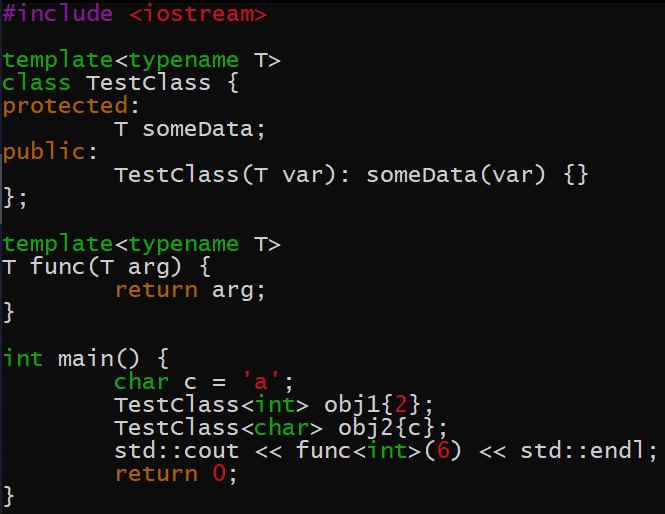
\includegraphics[width = 0.65\textwidth]{Шаблоны код.png}
    \caption{Шаблонизированные класс и фунция}
\end{figure}

\begin{figure}[H]\label{fig: Шаблонные классы}
    \subfloat[Конструктор класса с шаблоном \textit{int}]{
    \begin{minipage}[t]{0.5\textwidth}
        \centering
        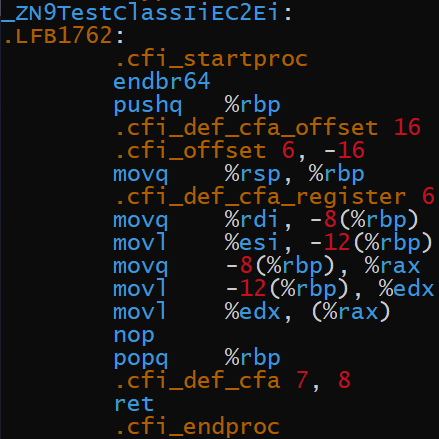
\includegraphics[scale = 0.55]{Шаблонный класс1 листинг.png}
    \end{minipage}}
    \subfloat[Конструктор класса с шаблоном \textit{char}]{
    \begin{minipage}[t]{0.5\textwidth}
        \centering
        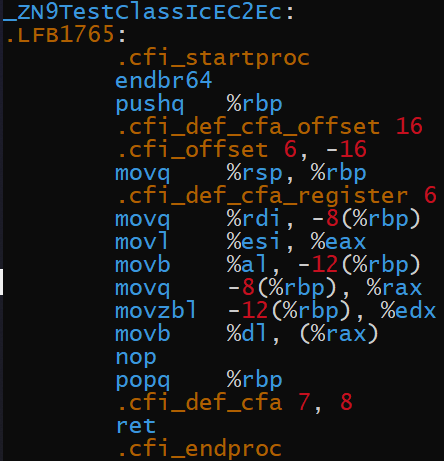
\includegraphics[scale = 0.525]{Шаблонный класс2 листинг.png}
    \end{minipage}}
\end{figure}
Получаем, что при создании экземпляра, когда шаблон раскрывается, компилятор создаёт конструктор и все функции, уже зная что будет вместо шаблона, поэтому объекты класса с различным раскрытием шаблонов как бы являются экземплярами различных классов. То есть генерируется столько различных классов, сколько было уникальных раскрытий шаблона. Это же видно и из названия конструктора. После названия класса идёт буква \textit{I}, что судя по всему указывает на то, что это шаблонный класс (или функция), потом идёт информация о том, что конкретно подставляется в шаблон, в конце, как и у обычных функций, указаны типы данных аргументов функции.  

\textbf{Пункт 11: \textit{Rvalue}-ссылки}

Ещё раз взглянем на \textit{rvalue}-ссылки в ассемблерном представлении.

\begin{figure}[H]\label{fig: ref и rvalue ref код}
    \centering
    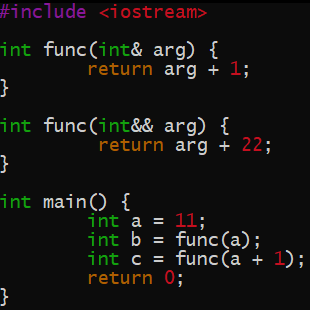
\includegraphics[width = 0.35\textwidth]{Rvalue-ссылки код.png}
    \caption{Функции, принимающие ссылку и \textit{rvalue}-ссылку}
\end{figure}

\begin{figure}[H]\label{fig: Названия ref и rvalue ref функций}
    \subfloat[Обычная ссылка]{
    \begin{minipage}[t]{0.4\textwidth}
        \centering
        
\includegraphics[scale = 0.6]{Функция ref название.png}
    \end{minipage}}
    \subfloat[\textit{Rvalue}-ссылка]{
    \begin{minipage}[t]{0.4\textwidth}
        \centering
        
\includegraphics[scale = 0.6]{Функция Rvalue-ref название.png}
    \end{minipage}}
\end{figure}
Как и должно быть в конце названия функции указан тип данных аргументов, в первом случае это обычная \textit{int} ссылка \textit{Ri}, \textit{rvalue}-ссылка на \textit{int} обозначается через \textit{Oi}. Перед вызовом функции с аргументом \textit{rvalue}-ссылкой результат промежуточной операции кладётся в стек как локальная переменная, затем уже через регистр передаётся в функцию, именно благодаря этому и можно экономить время, избегая глубокого копирования там, где оно не нужно.  

\textbf{Пункт 12: \textit{Enum}}

Посмотрим на конструкцию \textit{enum} в ассемблерном листинге.

\begin{figure}[H]\label{fig: Enum код и листинг}
    \subfloat[Код с \textit{enum} C++]{
    \begin{minipage}[t]{0.5\textwidth}
        \centering
        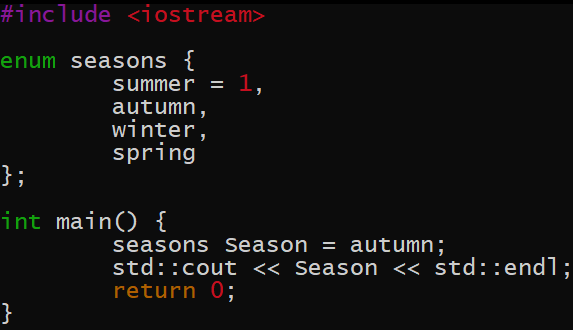
\includegraphics[scale = 0.5]{Enum код.png}
    \end{minipage}}
    \subfloat[Ассемблерный листинг программы]{
    \begin{minipage}[t]{0.5\textwidth}
        \centering
        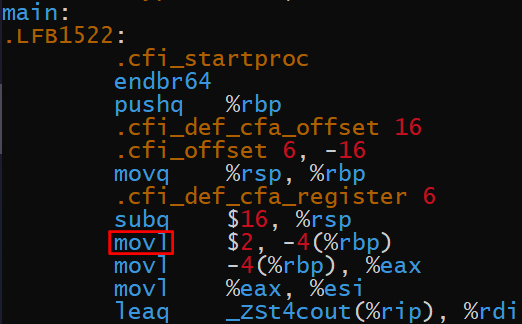
\includegraphics[scale = 0.505]{Enum листинг.png}
    \end{minipage}}
\end{figure}
Как видно из листинга, компилятор сам заменяет переменную на соответствующую ей числовую константу, то есть в ассемблерном листинге получаем переменную типа \textit{int} (в данном случае). 

\end{document}
